\chapter{Espectroscopia para a estrutura}\label{ch:b1:structure-spectroscopy}

Um perfumista entrega ao laboratório um líquido incolor com cheiro de
abacaxi e pergunta o que é. Há cinquenta anos, a resposta teria levado
semanas de reações de degradação. Hoje ela leva dez minutos: uma
análise elementar dá a fórmula, um espectro no infravermelho indica o
grupo funcional e um espectro de ressonância magnética nuclear de próton
mostra como os átomos estão ligados. Este capítulo explica como se lê
cada espectro --- o que a luz de cada região faz a uma molécula, e quais
características de um espectro trazem qual pedaço da estrutura --- e
termina com essa molécula de abacaxi.

\begin{recall}
O volume escolar (anos 11 e 12) mediu \omterm{def:b1:structure-spectroscopy:absorbance}{absorbâncias} com um
espectrofotômetro e usou a lei de Beer--Lambert para encontrar
concentrações, identificou grupos funcionais a partir de tabelas de
bandas no infravermelho e leu espectros simples de RMN de próton (número
de sinais, \omterm{def:b1:structure-spectroscopy:integration}{integração}, regra do $n + 1$). As ligações simples, duplas e
triplas e a ligação $\pi$ são as do \cref{ch:b1:lewis-resonance-vsepr}.
\end{recall}

\section{Espectroscopia UV--visível: conjugação e cor}

\begin{definition}[Absorbância e a lei de Beer--Lambert]\label{def:b1:structure-spectroscopy:absorbance}
Para uma luz de intensidade $I_0$ que entra em uma solução e $I$ que
sai dela, a \emph{absorbância}\index{absorbancia@absorbância} é $A = \log(I_0/I)$. Para uma
solução diluída de uma única espécie absorvente, $A = \varepsilon\,\ell\,c$
(a lei de Beer--Lambert), em que $\ell$ é o comprimento do percurso, $c$
a concentração e $\varepsilon$ o \emph{coeficiente de absorção
molar}\index{coeficiente de absorcao molar@coeficiente de absorção molar}, uma propriedade da espécie
nesse comprimento de onda.
\end{definition}

Uma molécula absorve luz ultravioleta ou visível quando a energia de um
fóton corresponde à diferença entre os níveis eletrônicos ocupado mais
alto e vazio mais baixo de suas ligações. Para as ligações $\sigma$, a
diferença é grande e a absorção fica muito dentro do ultravioleta; as
ligações $\pi$ absorvem mais perto do visível, e uma cadeia de ligações
duplas e simples alternadas absorve em comprimentos de onda tanto mais
longos quanto mais longa for a cadeia.

\begin{definition}[Sistema conjugado, cromóforo, máximo de absorção]\label{def:b1:structure-spectroscopy:conjugation}
Um \emph{sistema conjugado}\index{sistema conjugado} é uma cadeia de
átomos que levam, cada um, um orbital $p$ em um sistema $\pi$, como nas
ligações duplas e simples alternadas (buta-1,3-dieno, benzeno). O grupo
de átomos responsável por uma absorção é o seu
\emph{cromóforo}\index{cromoforo@cromóforo}; o comprimento de onda em que sua
\omterm{def:b1:structure-spectroscopy:absorbance}{absorbância} é máxima é o \emph{máximo de absorção}\index{maximo de absorcao@máximo de absorção},
$\lambda_{\max}$.
\end{definition}

Os níveis de um \omterm{def:b1:structure-spectroscopy:conjugation}{sistema conjugado} se espalham por toda a cadeia e se
aproximam à medida que a cadeia cresce, como os níveis de uma partícula
em uma caixa mais longa: $\lambda_{\max}$ aumenta com a conjugação. O
eteno e o butadieno só absorvem no ultravioleta; as onze ligações duplas
conjugadas do $\beta$-caroteno levam a absorção para a parte azul do
visível. Uma substância tem a cor complementar da luz que absorve:
absorvendo o azul e o violeta, o caroteno parece laranja.

\begin{omfigure}
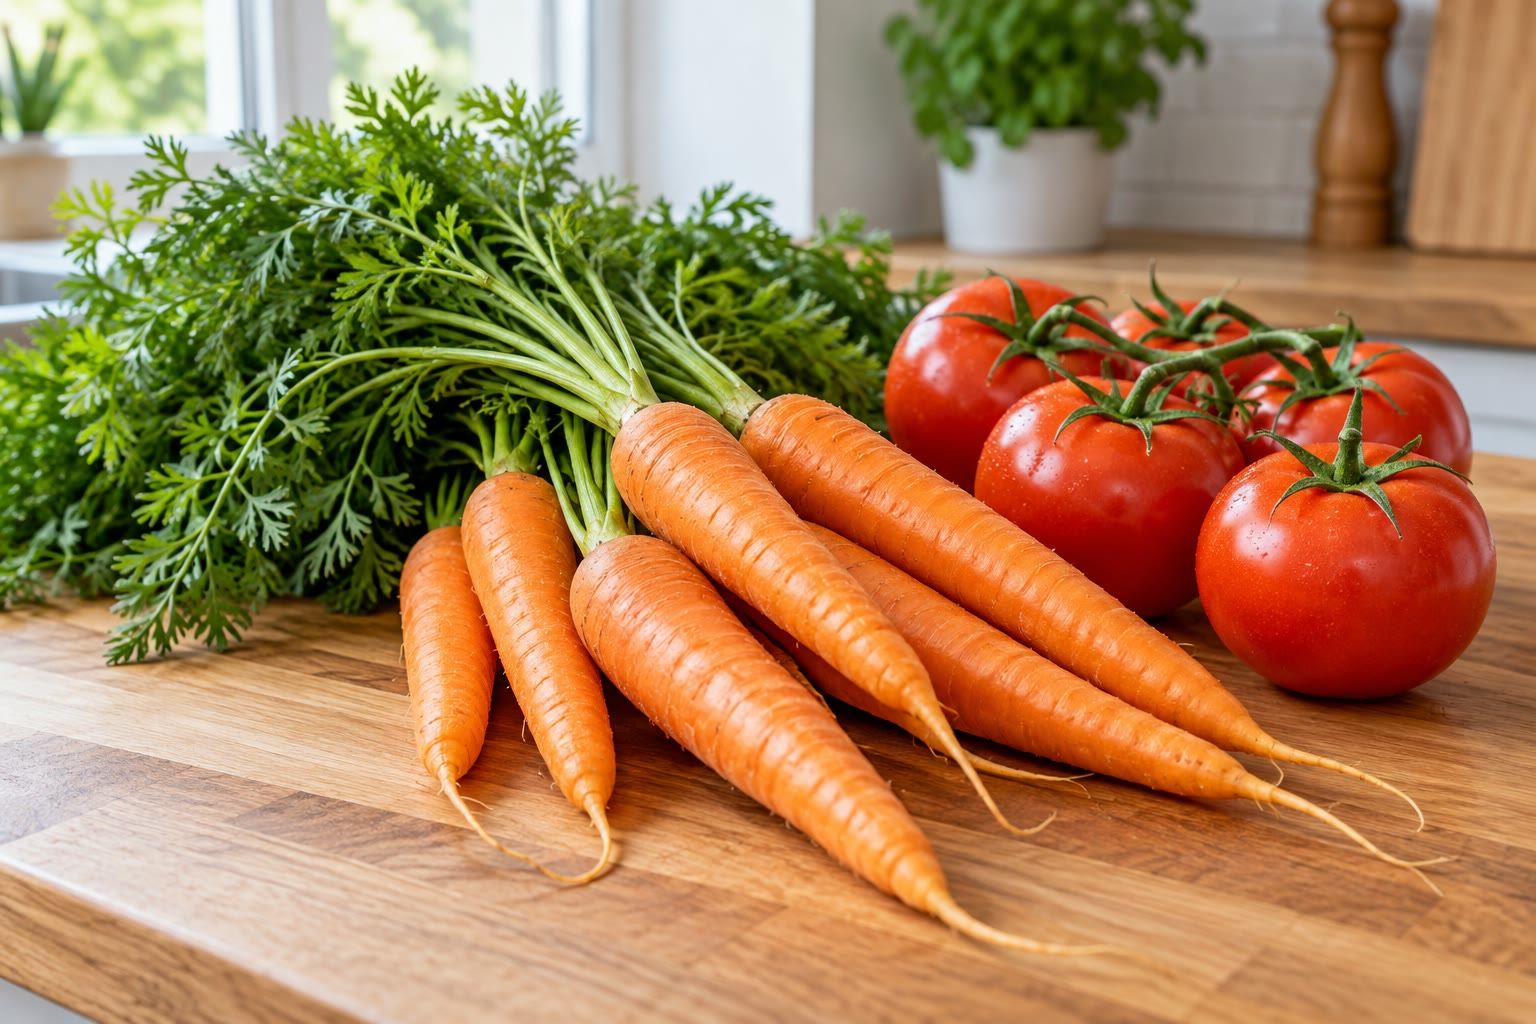
\includegraphics[width=0.55\linewidth]{images/book2/ai/b1-17-carrots-tomatoes.jpg}

{\small As cenouras e os tomates devem suas cores a longas moléculas
conjugadas, os carotenos e o licopeno, que absorvem a luz azul e verde e
deixam passar o laranja e o vermelho.}
\end{omfigure}

\begin{omfigure}
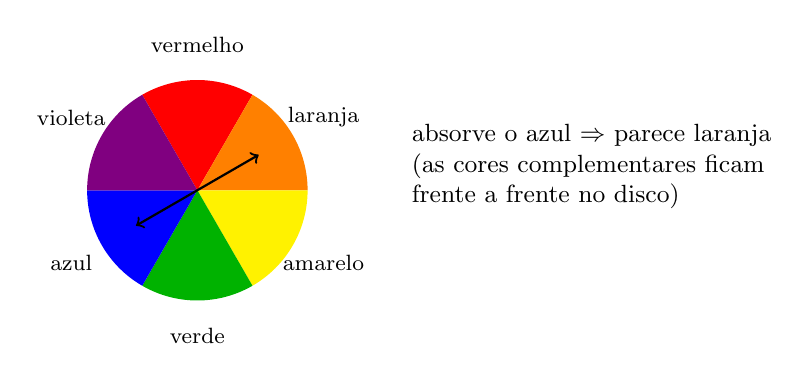
\begin{tikzpicture}[font=\small]
  \foreach \a/\c/\n in {90/red/{\footnotesize vermelho}, 30/orange/{\footnotesize laranja}, -30/yellow/{\footnotesize amarelo}, -90/green!70!black/{\footnotesize verde}, -150/blue/{\footnotesize azul}, 150/violet/{\footnotesize violeta}} {
    \fill[\c] (0,0) -- (\a-30:1.4) arc[start angle=\a-30, end angle=\a+30, radius=1.4] -- cycle;
    \node at (\a:1.85) {\n};
  }
  \draw[<->, thick] (-150:0.9) -- (30:0.9);
  \node[align=left, anchor=west] at (2.6,0.3) {absorve o azul $\Rightarrow$ parece laranja\\(as cores complementares ficam\\frente a frente no disco)};
\end{tikzpicture}

{\small Um disco de cores. A cor vista é o complemento da cor absorvida:
uma solução que absorve no azul parece laranja.}
\end{omfigure}

\section{A espectroscopia no infravermelho aprofundada}

\begin{definition}[Número de onda, transmitância, região de impressão digital]\label{def:b1:structure-spectroscopy:wavenumber}
Os espectros no infravermelho são traçados em função do \emph{número de
onda}\index{numero de onda@número de onda} $\tilde\nu = 1/\lambda$, em \unit{cm^{-1}},
proporcional à energia do fóton. A ordenada é a
\emph{transmitância}\index{transmitancia@transmitância} $T = I/I_0$, em porcentagem, de modo
que as bandas apontam para baixo. Abaixo de cerca de
\qty{1500}{cm^{-1}}, muitas bandas sobrepostas, características da
molécula inteira e não de uma ligação, formam a \emph{região de
impressão digital}\index{regiao de impressao digital@região de impressão digital}.
\end{definition}

Uma ligação absorve a luz infravermelha na frequência em que vibra. Como
para duas massas ligadas por uma mola, quanto mais rígida a ligação e
mais leves os átomos, maior o \omterm{def:b1:structure-spectroscopy:wavenumber}{número de onda}: ligações com o hidrogênio
(O--H, C--H) acima de \qty{2800}{cm^{-1}}, ligações triplas perto de
2200, ligações duplas perto de 1700--1600, ligações simples entre átomos
mais pesados abaixo de 1300. A tabela dá posições medidas para as
moléculas deste capítulo, em \omterm{def:b1:extent-q-and-k:system}{fase} gasosa, onde as moléculas estão
isoladas.
\begin{omfigure}
\begin{tabular}{llr}
\hline
molécula & ligação & $\tilde\nu$ (\unit{cm^{-1}}) \\
\hline
etanol & O--H & 3666 \\
etanol & C--H & 2978 \\
etanol & C--O & 1060 \\
propanona & C=O & 1738 \\
ácido etanoico & O--H & 3582 \\
ácido etanoico & C=O & 1788 \\
etanoato de etila & C=O & 1764 \\
etanoato de etila & C--O & 1238 \\
\hline
\end{tabular}

\smallskip
{\small Máximos de banda em espectros no infravermelho em \omterm{def:b1:extent-q-and-k:system}{fase} gasosa.
Nos líquidos, as \omterm{def:b1:intermolecular-forces-solvents:hbond}{ligações de hidrogênio} alargam as bandas O--H e as
deslocam para \omterm{def:b1:structure-spectroscopy:wavenumber}{números de onda} menores, e as bandas C=O dos ácidos
descem à medida que o ácido se emparelha.}
% ledger: ir:ethanol-OH, ir:ethanol-CH, ir:ethanol-CO, ir:propanone-CO, ir:ethanoic-OH, ir:ethanoic-CO, ir:ethylethanoate-CO, ir:ethylethanoate-COC
\end{omfigure}

\begin{omfigure}
\begin{tikzpicture}
\begin{axis}[name=i1, width=0.86\linewidth, height=3.2cm, xmin=500, xmax=4000, x dir=reverse, ymin=0, ymax=105, ytick={0,50,100}, ylabel={$T$ (\%)}, tick label style={font=\scriptsize}, label style={font=\small}, xticklabels={}]
\addplot[omDef, thick] table[x=nu, y=T] {figdata/out/bachelor-1-spectra-ir-ethanol.dat};
\node[font=\scriptsize, anchor=west] at (axis cs:2600,25) {etanol};
\end{axis}
\begin{axis}[name=i2, at={(i1.south)}, anchor=north, yshift=-0.25cm, width=0.86\linewidth, height=3.2cm, xmin=500, xmax=4000, x dir=reverse, ymin=0, ymax=105, ytick={0,50,100}, ylabel={$T$ (\%)}, tick label style={font=\scriptsize}, label style={font=\small}, xticklabels={}]
\addplot[omProp, thick] table[x=nu, y=T] {figdata/out/bachelor-1-spectra-ir-propanone.dat};
\node[font=\scriptsize, anchor=west] at (axis cs:2600,25) {propanona};
\end{axis}
\begin{axis}[at={(i2.south)}, anchor=north, yshift=-0.25cm, width=0.86\linewidth, height=3.2cm, xmin=500, xmax=4000, x dir=reverse, ymin=0, ymax=105, ytick={0,50,100}, ylabel={$T$ (\%)}, tick label style={font=\scriptsize}, label style={font=\small}, xlabel={número de onda (\unit{cm^{-1}})}]
\addplot[omMeth, thick] table[x=nu, y=T] {figdata/out/bachelor-1-spectra-ir-ethanoic.dat};
\node[font=\scriptsize, anchor=west] at (axis cs:2600,25) {ácido etanoico};
\end{axis}
\end{tikzpicture}

{\small Espectros no infravermelho do etanol, da propanona e do ácido
etanoico, simulados a partir das posições de banda medidas da tabela
(alturas e larguras das bandas esquemáticas). A banda C=O perto de
\qty{1750}{cm^{-1}} e a banda O--H acima de \qty{3500}{cm^{-1}}
distinguem os três grupos funcionais à primeira vista.}
\end{omfigure}

\section{RMN de próton: deslocamento químico e integração}

Em um campo magnético intenso, um próton tem dois \omterm{def:b1:quantum-numbers:energy-level}{níveis de energia};
ondas de rádio de frequência adequada o fazem passar de um ao outro.
Essa frequência é proporcional ao campo magnético que o próton
efetivamente sente, que os elétrons à sua volta reduzem ligeiramente.
Prótons em ambientes químicos diferentes ressoam, portanto, em
frequências ligeiramente diferentes.

\begin{definition}[Deslocamento químico, blindagem, prótons equivalentes]\label{def:b1:structure-spectroscopy:chemical-shift}
O \emph{deslocamento químico}\index{deslocamento quimico@deslocamento químico} de um próton é
$\delta = (\nu - \nu_{\text{ref}})/\nu_0 \times 10^6$, em \unit{ppm}, em que
$\nu$ é sua frequência de ressonância, $\nu_{\text{ref}}$ a dos prótons
do tetrametilsilano e $\nu_0$ a frequência de operação do
espectrômetro. A redução do campo em um núcleo por seus elétrons é a sua
\emph{blindagem magnética}\index{blindagem magnetica@blindagem magnética}: vizinhos retiradores de
elétrons (O, halogênios, C=O) desblindam um próton e aumentam seu
$\delta$. \emph{Prótons equivalentes}\index{protons equivalentes@prótons equivalentes} são prótons
trocados entre si por uma simetria da molécula ou por uma rotação
rápida; eles têm o mesmo deslocamento.
\end{definition}

\begin{proposition}[O deslocamento não depende do espectrômetro]\label{prop:b1:structure-spectroscopy:shift-field-independent}
O \omterm{def:b1:structure-spectroscopy:chemical-shift}{deslocamento químico} de um próton é o mesmo em espectrômetros de
campos diferentes.
\end{proposition}

\begin{proof}
Tanto $\nu$ quanto $\nu_{\text{ref}}$ são proporcionais ao campo
aplicado $B_0$ (cada um multiplicado por seu próprio fator de
blindagem), assim como $\nu_0$. A razão $(\nu - \nu_{\text{ref}})/\nu_0$
é, portanto, independente de $B_0$. As diferenças em hertz, ao
contrário, crescem com o campo.
\end{proof}

\begin{definition}[Integração]\label{def:b1:structure-spectroscopy:integration}
A \emph{integração}\index{integracao@integração} de um sinal é a sua área, lida no
espectro como a altura de uma curva em degraus; as áreas são
proporcionais aos números de prótons que dão os sinais.
\end{definition}

\section{O acoplamento spin--spin}

\begin{definition}[Acoplamento spin--spin, constante de acoplamento, multipleto]\label{def:b1:structure-spectroscopy:coupling}
Através das ligações, o estado magnético de um próton altera
ligeiramente o campo sentido pelos prótons dos carbonos vizinhos: esse
\emph{acoplamento spin--spin}\index{acoplamento spin--spin} desdobra cada sinal em
um \emph{multipleto}\index{multipleto} de linhas separadas pela
\emph{constante de acoplamento}\index{constante de acoplamento} $J$, em hertz. Dois
prótons acoplados entre si mostram o mesmo $J$; \omterm{def:b1:structure-spectroscopy:chemical-shift}{prótons equivalentes} não
desdobram o sinal um do outro.
\end{definition}

\begin{proposition}[A regra do \texorpdfstring{$n + 1$}{n + 1}]\label{prop:b1:structure-spectroscopy:n-plus-one}
Um próton (ou um conjunto de \omterm{def:b1:structure-spectroscopy:chemical-shift}{prótons equivalentes}) acoplado com o mesmo
$J$ a $n$ vizinhos equivalentes dá $n + 1$ linhas, separadas por $J$, de
intensidades relativas iguais aos coeficientes binomiais $\binom{n}{k}$,
$k = 0$ a $n$ (a \emph{regra do $n + 1$}\index{regra do $n + 1$}).
\end{proposition}

\begin{proof}
Cada vizinho está em um de dois estados de spin, deslocando a linha
observada de $+J/2$ ou de $-J/2$. Com $n$ vizinhos, o deslocamento é
$(k - n/2)J$, em que $k$ é o número deles no primeiro estado: $n + 1$
valores, igualmente espaçados de $J$. Como os dois estados estão quase
igualmente povoados, todas as $2^n$ combinações são igualmente
prováveis, e ter $k$ delas no primeiro estado acontece de $\binom{n}{k}$
maneiras.
\end{proof}

\begin{omfigure}
\begin{tikzpicture}[font=\small, x=0.85cm, y=0.5cm]
  % quartet: three neighbours, each split +-J/2 (J = 1.5 units)
  \draw[thick] (0,4) -- (0,3.4);
  \foreach \x in {-0.75,0.75} \draw (0,3.4) -- (\x,2.4);
  \foreach \a/\b in {-0.75/-1.5, -0.75/0, 0.75/0, 0.75/1.5} \draw (\a,2.4) -- (\b,1.4);
  \foreach \a/\b in {-1.5/-2.25, -1.5/-0.75, 0/-0.75, 0/0.75, 1.5/0.75, 1.5/2.25} \draw (\a,1.4) -- (\b,0.4);
  \foreach \x/\h in {-2.25/1, -0.75/3, 0.75/3, 2.25/1} {\draw[omDef, very thick] (\x,-2.6) -- (\x,{-2.6+0.7*\h}); \draw[dotted] (\x,0.4) -- (\x,{-2.6+0.7*\h});}
  \draw (-2.8,-2.6) -- (2.8,-2.6);
  \node at (0,-3.4) {quarteto 1\,:\,3\,:\,3\,:\,1 (\ce{-CH2-} vizinho de \ce{-CH3})};
  % triplet: two neighbours
  \begin{scope}[xshift=7.5cm]
  \draw[thick] (0,4) -- (0,3.4);
  \foreach \x in {-0.75,0.75} \draw (0,3.4) -- (\x,2.4);
  \foreach \a/\b in {-0.75/-1.5, -0.75/0, 0.75/0, 0.75/1.5} \draw (\a,2.4) -- (\b,1.4);
  \foreach \x/\h in {-1.5/1, 0/2, 1.5/1} {\draw[omProp, very thick] (\x,-2.6) -- (\x,{-2.6+0.7*\h}); \draw[dotted] (\x,1.4) -- (\x,{-2.6+0.7*\h});}
  \draw (-2.1,-2.6) -- (2.1,-2.6);
  \draw[<->] (-1.5,-0.6) -- (0,-0.6) node[midway, above, font=\scriptsize] {$J$};
  \node at (0,-3.4) {tripleto 1\,:\,2\,:\,1 (\ce{-CH3} vizinho de \ce{-CH2-})};
  \end{scope}
\end{tikzpicture}

{\small Árvores de desdobramento. Cada vizinho desdobra cada linha em
duas, separadas por $J$; as linhas que coincidem se somam, dando as
intensidades binomiais.}
\end{omfigure}

\begin{omfigure}
\begin{tikzpicture}
\begin{axis}[name=ea,
  width=0.86\linewidth, height=4.2cm, xmin=0.8, xmax=4.5, x dir=reverse, ymin=0, ymax=1.15,
  axis x line=bottom, axis y line=none, xlabel={$\delta$ (ppm)},
  tick label style={font=\scriptsize}, label style={font=\small}]
\addplot[omDef, thin] table[x=ppm, y=I] {figdata/out/bachelor-1-spectra-nmr-ethylethanoate.dat};
\node[font=\scriptsize, anchor=south] at (axis cs:4.12,0.75) {q, 2H};
\node[font=\scriptsize, anchor=west] at (axis cs:2.0,0.95) {s, 3H};
\node[font=\scriptsize, anchor=west] at (axis cs:1.15,0.8) {t, 3H};
\node[font=\small, anchor=north] at (axis cs:3.0,1.1) {\ce{CH3COOCH2CH3}};
\end{axis}
\begin{axis}[at={(ea.south)}, anchor=north, yshift=-1.3cm,
  width=0.86\linewidth, height=4.2cm, xmin=0.8, xmax=4.5, x dir=reverse, ymin=0, ymax=1.15,
  axis x line=bottom, axis y line=none, xlabel={$\delta$ (ppm)},
  tick label style={font=\scriptsize}, label style={font=\small}]
\addplot[omProp, thin] table[x=ppm, y=I] {figdata/out/bachelor-1-spectra-nmr-ethanol.dat};
\node[font=\scriptsize, anchor=south] at (axis cs:3.69,0.75) {q, 2H};
\node[font=\scriptsize, anchor=west] at (axis cs:2.55,0.6) {s, 1H};
\node[font=\scriptsize, anchor=west] at (axis cs:1.1,0.8) {t, 3H};
\node[font=\small, anchor=north] at (axis cs:2.9,1.1) {\ce{CH3CH2OH}};
\end{axis}
\end{tikzpicture}

{\small Espectros de RMN de próton do etanoato de etila (em cima) e do
etanol (embaixo) em \ce{CDCl3}, simulados a \qty{90}{MHz} a partir de
deslocamentos e \omterm{def:b1:structure-spectroscopy:coupling}{constantes de acoplamento} medidos ($J = \qty{7.2}{Hz}$ e
\qty{7.0}{Hz}). O quarteto de \ce{OCH2} é desblindado pelo oxigênio; no
etanol, o próton do OH, trocado rapidamente entre as moléculas, não se
acopla, e seu deslocamento depende da concentração.}
% ledger: nmr:ethylethanoate-OCH2, nmr:ethylethanoate-COCH3, nmr:ethylethanoate-CH3, nmr:ethylethanoate-J, nmr:ethanol-CH2, nmr:ethanol-CH3, nmr:ethanol-OH, nmr:ethanol-J
\end{omfigure}

\begin{omfigure}
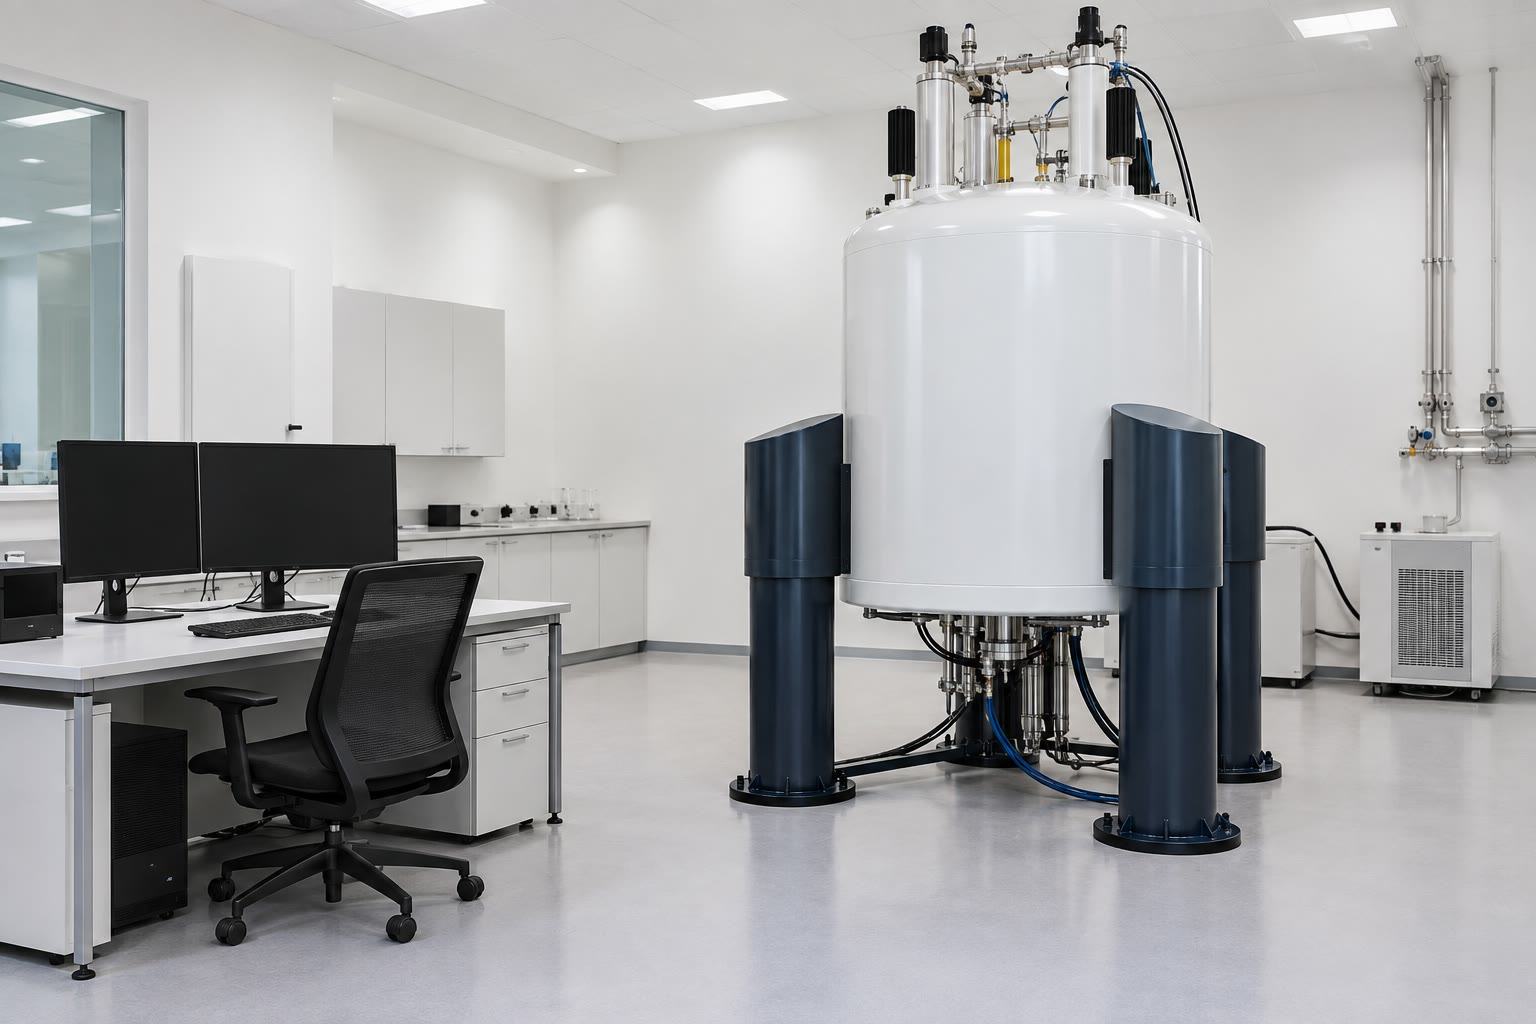
\includegraphics[width=0.5\linewidth]{images/book2/ai/b1-17-nmr.jpg}

{\small Um espectrômetro de RMN: o cilindro alto abriga um ímã
supercondutor resfriado com hélio líquido; o tubo da amostra desce até
o seu centro.}
\end{omfigure}

\section{Resolver uma estrutura}

\begin{definition}[Grau de insaturação]\label{def:b1:structure-spectroscopy:unsaturation}
O \emph{grau de insaturação}\index{grau de insaturacao@grau de insaturação} de uma fórmula
é o número de anéis mais o número de ligações $\pi$ da molécula.
\end{definition}

\begin{proposition}[Grau de insaturação a partir da fórmula]\label{prop:b1:structure-spectroscopy:unsaturation-formula}
Para uma molécula $\mathrm{C}_c\mathrm{H}_h\mathrm{N}_n\mathrm{O}_o\mathrm{X}_x$
(X um halogênio), o \omterm{def:b1:structure-spectroscopy:unsaturation}{grau de insaturação} é
\[
  D = \frac{2c + 2 + n - h - x}{2} .
\]
\end{proposition}

\begin{proof}
Uma cadeia aberta de $c$ carbonos só com ligações simples leva $2c + 2$
hidrogênios. Cada anel ou ligação $\pi$ retira dois deles. Um oxigênio
divalente inserido em uma cadeia não muda nada; um nitrogênio trivalente
traz um hidrogênio a mais; um halogênio toma o lugar de um hidrogênio.
Contar os hidrogênios que faltam e dividir por dois dá $D$.
\end{proof}

\begin{method}[Resolver uma estrutura]\label{met:b1:structure-spectroscopy:solve-structure}
\begin{enumerate}
  \item A partir da fórmula, calcule $D$.
  \item A partir do espectro no infravermelho, encontre os grupos
        funcionais (C=O, O--H, N--H, C--O) e a ausência de outros.
  \item A partir do espectro de RMN: número de sinais (conjuntos de
        \omterm{def:b1:structure-spectroscopy:chemical-shift}{prótons equivalentes}), \omterm{def:b1:structure-spectroscopy:integration}{integrações} (prótons por conjunto),
        deslocamentos (grupos vizinhos), \omterm{def:b1:crystals-metals:multiplicity}{multiplicidades} (número de
        vizinhos pela regra do $n + 1$), \omterm{def:b1:structure-spectroscopy:coupling}{constantes de acoplamento} (quais
        sinais são vizinhos).
  \item Monte fragmentos, una-os e confira cada pico com a estrutura
        proposta; descarte os isômeros que não concordam.
\end{enumerate}
\end{method}

\section{Exercícios}

\begin{exercise}[$\star$]\label{exo:b1:structure-spectroscopy:1}
Uma solução de um corante a \qty{2.0e-5}{mol/L} em uma cubeta de
\qty{1.00}{cm} tem \omterm{def:b1:structure-spectroscopy:absorbance}{absorbância} de 0.64 em seu \omterm{def:b1:structure-spectroscopy:conjugation}{máximo de absorção}. Calcule
$\varepsilon$ e a \omterm{def:b1:structure-spectroscopy:absorbance}{absorbância} de uma solução três vezes mais
concentrada.
\end{exercise}

\begin{exercise}[$\star$]\label{exo:b1:structure-spectroscopy:2}
Calcule o \omterm{def:b1:structure-spectroscopy:unsaturation}{grau de insaturação} de \ce{C6H6}, \ce{C4H8O2}, \ce{C3H7NO},
\ce{C2H3Cl} e \ce{C10H14O} (carvona). Proponha uma estrutura para cada um.
\end{exercise}

\begin{exercise}[$\star$]\label{exo:b1:structure-spectroscopy:3}
Quantos sinais de próton, com quais \omterm{def:b1:structure-spectroscopy:integration}{integrações}, dão a propanona, o
ácido etanoico, o 2-metilpropano e o 1,2-dicloroetano?
\end{exercise}

\begin{exercise}[$\star$]\label{exo:b1:structure-spectroscopy:4}
Um sinal fica a \qty{1460}{Hz} do tetrametilsilano em um espectrômetro
de \qty{400}{MHz}. Qual é seu deslocamento? A quantos hertz ele estaria a
\qty{90}{MHz}? Por que os campos altos separam melhor os \omterm{def:b1:structure-spectroscopy:coupling}{multipletos}?
\end{exercise}

\begin{exercise}[$\star\star$]\label{exo:b1:structure-spectroscopy:5}
Preveja a multiplicidade de cada sinal do 1-bromopropano,
\ce{CH3CH2CH2Br}, supondo \omterm{def:b1:structure-spectroscopy:coupling}{constantes de acoplamento} iguais, e as
intensidades relativas das linhas do sinal central.
\end{exercise}

\begin{exercise}[$\star\star$]\label{exo:b1:structure-spectroscopy:6}
Em que diferem os espectros no infravermelho do etanol, da propanona e do
ácido etanoico entre 1700 e \qty{3700}{cm^{-1}}? Qual composto dá ao
mesmo tempo uma banda C=O e uma banda O--H?
\end{exercise}

\begin{exercise}[$\star\star$]\label{exo:b1:structure-spectroscopy:7}
Dois isômeros \ce{C4H8O2}: o etanoato de etila e o propanoato de metila.
Preveja seus espectros de RMN (deslocamentos aproximados,
\omterm{def:b1:crystals-metals:multiplicity}{multiplicidades}, \omterm{def:b1:structure-spectroscopy:integration}{integrações}) e diga como distingui-los.
\end{exercise}

\begin{exercise}[$\star\star$]\label{exo:b1:structure-spectroscopy:8}
Usando o espectro simulado do etanoato de etila, leia a separação de duas
linhas do quarteto em ppm e converta-a em hertz (o espectro é simulado a
\qty{90}{MHz}). Compare com o tripleto.
\end{exercise}

\begin{exercise}[$\star\star$]\label{exo:b1:structure-spectroscopy:9}
Um composto \ce{C3H6O} mostra uma banda forte no infravermelho em
\qty{1738}{cm^{-1}} e um único sinal de RMN. Identifique-o. Que isômero
mostraria uma banda perto de \qty{2720}{cm^{-1}} e um sinal perto de
\qty{9.8}{ppm}?
\end{exercise}

\begin{exercise}[$\star\star\star$]\label{exo:b1:structure-spectroscopy:10}
Demonstre a regra do $n + 1$ na forma: um próton acoplado a dois
conjuntos diferentes de vizinhos, $n_1$ com $J_1$ e $n_2$ com $J_2$, dá
$(n_1 +
1)(n_2 + 1)$ linhas. Quando $J_1 = J_2$, quantas linhas distintas
restam? Aplique ao \ce{CH2} central do 1-bromopropano.
\end{exercise}

\begin{exercise}[$\star\star\star$]\label{exo:b1:structure-spectroscopy:11}
Um composto \ce{C4H10O} não dá nenhuma banda no infravermelho entre 1700
e 1800, mas uma banda larga perto de \qty{3350}{cm^{-1}} no líquido, e um
espectro de RMN com um dubleto (6H), um \omterm{def:b1:structure-spectroscopy:coupling}{multipleto} (1H), um dubleto (2H)
e um singleto largo (1H). Encontre a estrutura.
\end{exercise}

\begin{exercise}[$\star\star\star$]\label{exo:b1:structure-spectroscopy:12}
Mostre que a \omterm{def:b1:structure-spectroscopy:absorbance}{absorbância} de uma mistura de duas espécies obedece a
$A = \ell(\varepsilon_1c_1
+ \varepsilon_2c_2)$, e explique como medidas em dois comprimentos de onda
dão as duas concentrações.
\end{exercise}

\section{Problema: A molécula do abacaxi}

\begin{problem}[{Problema de fim de semana --- a análise por combustão e a
densidade do vapor, o espectro no infravermelho, o espectro de RMN de
próton, e a estrutura e a massa molar do éster com cheiro de abacaxi}]
\label{pb:b1:structure-spectroscopy:1}
A incógnita é um líquido que contém apenas C, H e O. A combustão de
\qty{0.2500}{g} dá \qty{0.5690}{g} de dióxido de carbono e
\qty{0.2328}{g} de água. Seu vapor tem densidade de \qty{3.74}{g/L} a
\qty{100}{\celsius} e \qty{1.000}{bar}. Bandas no infravermelho em \omterm{def:b1:extent-q-and-k:system}{fase}
gasosa: 2982, 1754, \qty{1182}{cm^{-1}} (forte), nenhuma acima de
\qty{3100}{cm^{-1}}. RMN de próton (\ce{CDCl3}): 4.13 (q, 2H, $J = \qty{7.2}{Hz}$),
2.28 (t, 2H), 1.66 (sexteto, 2H), 1.25 (t, 3H, $J = \qty{7.2}{Hz}$), 0.95
(t, 3H) ppm. $M$: C 12.0, H 1.0, O \qty{16.0}{g/mol}; $R =
\qty{8.314}{J/(K.mol)}$.
% ledger: ir:ethylbutanoate-CH, ir:ethylbutanoate-CO, ir:ethylbutanoate-COC, nmr:ethylbutanoate-OCH2, nmr:ethylbutanoate-CH2CO, nmr:ethylbutanoate-CH2, nmr:ethylbutanoate-OCH2CH3, nmr:ethylbutanoate-CH3, nmr:ethylbutanoate-J

\begin{center}
\begin{tikzpicture}
\begin{axis}[width=0.86\linewidth, height=4.0cm, xmin=0.6, xmax=4.5, x dir=reverse, ymin=0, ymax=1.15,
  axis x line=bottom, axis y line=none, xlabel={$\delta$ (ppm)},
  tick label style={font=\scriptsize}, label style={font=\small}]
\addplot[omDef, thin] table[x=ppm, y=I] {figdata/out/bachelor-1-spectra-nmr-ethylbutanoate.dat};
\end{axis}
\end{tikzpicture}
\end{center}

\medskip
\noindent\textbf{Parte I --- A fórmula.}
\begin{enumerate}
  \item Calcule a massa de carbono na amostra.
  \item Calcule a massa de hidrogênio.
  \item Deduza a massa de oxigênio.
  \item Calcule as porcentagens em massa de C, H e O.
  \item Encontre a fórmula empírica.
  \item A partir da densidade do vapor, calcule a massa molar (gás ideal).
  \item Dê a fórmula molecular e seu \omterm{def:b1:structure-spectroscopy:unsaturation}{grau de insaturação}.
\end{enumerate}

\medskip
\noindent\textbf{Parte II --- O espectro no infravermelho.}
\begin{enumerate}[resume]
  \item Atribua a banda em \qty{1754}{cm^{-1}}.
  \item O que a ausência de bandas acima de \qty{3100}{cm^{-1}} exclui?
  \item Atribua a banda forte em \qty{1182}{cm^{-1}}.
  \item Atribua a banda em \qty{2982}{cm^{-1}}.
  \item Com o \omterm{def:b1:structure-spectroscopy:unsaturation}{grau de insaturação}, que família de compostos resta? Por
        que não um ácido carboxílico, uma cetona com um éter ou um diol
        cíclico?
\end{enumerate}

\medskip
\noindent\textbf{Parte III --- O espectro de RMN.}
\begin{enumerate}[resume]
  \item Quantos conjuntos de \omterm{def:b1:structure-spectroscopy:chemical-shift}{prótons equivalentes}? Verifique a \omterm{def:b1:structure-spectroscopy:integration}{integração}
        total.
  \item Interprete o quarteto em 4.13 ppm: vizinhos e ambiente.
  \item Interprete o tripleto em 1.25 ppm. Por que os dois têm o mesmo
        $J$?
  \item Interprete o tripleto em 2.28 ppm.
  \item Interprete o sexteto em 1.66 ppm.
  \item Interprete o tripleto em 0.95 ppm.
  \item Monte os dois fragmentos que esses sinais descrevem.
  \item Por que os sinais em 4.13 e 2.28 ppm são os mais desblindados?
\end{enumerate}

\medskip
\noindent\textbf{Parte IV --- A estrutura.}
\begin{enumerate}[resume]
  \item Una os fragmentos pelo grupo éster: duas possibilidades. Qual é
        compatível com os deslocamentos?
  \item Explique por que o propanoato de propila não serve.
  \item Explique por que o etanoato de butila não serve.
  \item Dê o nome do composto e desenhe sua estrutura.
  \item Verifique cada banda no infravermelho e cada sinal de RMN em
        relação à estrutura.
  \item Indique a massa molar da molécula do abacaxi.
\end{enumerate}
\end{problem}
